\documentclass[journal]{IEEEtran}

% ===== Packages =====
\usepackage{amsmath,amssymb,amsfonts}
\usepackage{graphicx}
\usepackage{booktabs}
\usepackage[caption=false,font=footnotesize]{subfig}
\usepackage{cite}
\usepackage{url}

% ★ フォント(Times 系に統一 & XeTeX 警告回避)
\usepackage{newtxtext,newtxmath}

% TikZ(図の描画用)
\usepackage{tikz}
\usetikzlibrary{arrows.meta,positioning,fit,backgrounds,calc,shadows.blur}
% ★ hyperref は最後に(IEEEtran 向け設定)
\usepackage{hyperref}

\hypersetup{
  colorlinks=false,           % IEEEtran は基本モノクロ
  pdfborder={0 0 0},          % リンク枠なし
  pdfauthor={Shinichi Samizo},
  pdftitle={Cross-Node Humanoid Robot Control: FSM, PID, State-Space and LLM Integration}
}

% ===== 図フォルダ =====
\graphicspath{{figures/}}

% ===== Document =====
\begin{document}

% ===== Title and Author =====
\title{Cross-Node Humanoid Robot Control: FSM, PID, State-Space and LLM Integration}

\author{Shinichi Samizo,~\IEEEmembership{Member,~IEEE}}

\maketitle

% ===== Author Note (全幅で出す) =====
\IEEEaftertitletext{%
\vspace{-1.2\baselineskip}%
\noindent\begin{minipage}{\textwidth}
\footnotesize
Shinichi Samizo is an independent semiconductor researcher and former engineer at Seiko Epson Corporation.\\[0.3em]
\textbf{Contact:} \href{mailto:shin3t72@gmail.com}{shin3t72@gmail.com} \quad
\textbf{GitHub:} \href{https://github.com/Samizo-AITL}{Samizo-AITL}
\end{minipage}%
\par\addvspace{0.8\baselineskip}%
}

% ===== Abstract & Keywords =====
\begin{abstract}
This paper presents a flagship proof-of-concept humanoid robot control system that integrates
finite state machines (FSM), proportional-integral-derivative (PID) controllers, state-space methods
(LQR/LQG), and large language models (LLMs) into a unified three-layer architecture. 
Unlike existing humanoid platforms such as Boston Dynamics Atlas and Tesla Optimus,
our approach emphasizes autonomy, fault tolerance, and sustainability.

The proposed architecture is realized as a cross-node chipset design: 
a 22 nm SoC executes LLM inference, FSM management, and state-space control;
a 0.18 µm AMS sensor hub processes multimodal inputs (vision, IMU, force, audio);
and a 0.35 µm LDMOS power drive with external GaN/MOSFET chips delivers high-torque actuation.
Energy harvesting via piezoelectric, photovoltaic, and regenerative methods 
extends operational lifetime in off-grid environments.

System-level modeling and verification are performed using SystemDK, 
demonstrating posture recovery within 200 ms, gait stability improved by 30\% over PID-only control,
and energy efficiency gains of 15\% with hybrid control and harvesting. 
Checkpointing with FRAM/EEPROM further enables fast resume ($\leq$10 ms) and robust mission continuity. 
These results highlight the feasibility of a sustainable and resilient humanoid control system
that bridges advanced control theory with emerging AI techniques.

\end{abstract}

\begin{IEEEkeywords}
Humanoid Robots, Fault-Tolerant Control, FSM, PID, State-Space Methods, LLM, Energy Harvesting
\end{IEEEkeywords}

% ===== Main Sections =====
\section{Introduction}

In the late 1990s, Japan's semiconductor industry was in transition. At Epson's Sakata 8-inch fab, DRAM was \emph{not} pursued as an end business; rather, DRAM technology transfer was used as a \textbf{strategic vehicle} to absorb submicron process technologies at and beyond 0.35~\si{\micro\meter} and redeploy them into Epson's core devices (ASICs, logic ICs, display drivers, and inkjet driver ICs).

The technology transfer from Mitsubishi covered three nodes, each with a clear role:
(1) 0.5~\si{\micro\meter} 16~Mbit DRAM --- to establish mass-production capability and stabilize fab operation; 
(2) 0.35~\si{\micro\meter} 64~Mbit DRAM (2nd gen) --- to introduce a scaled process while tackling yield window narrowing; 
(3) 0.25~\si{\micro\meter} 64~Mbit DRAM (3rd gen) --- as the next-stage validation bed and the basis for in-house deployment.

This paper focuses on the 0.25~\si{\micro\meter} (3rd gen) ramp-up in 1998: a process overview, the ramp-up method, and a failure-analysis–driven yield-improvement cycle. We also trace how these results enabled the 0.25~\si{\micro\meter} mobile pseudo-SRAM (VSRAM) in 2001 and why trench-based 0.18~\si{\micro\meter} VSRAM was abandoned.

\section{Related Work}
Classical humanoid control has relied heavily on PID loops
for joint-level stabilization and trajectory tracking.
Atlas, developed by Boston Dynamics, emphasizes highly dynamic behaviors
such as jumping and flipping through advanced mechanical design
and optimized low-level control.
Tesla's Optimus, in contrast, targets scalable production for industrial assistance,
focusing on simplified walking and manipulation tasks.

Beyond traditional approaches, state-space control methods,
including linear quadratic regulator (LQR) and linear quadratic Gaussian (LQG),
have been applied to multi-input multi-output humanoid stabilization problems.
More recently, integration of AI techniques such as reinforcement learning
has been explored to enhance adaptability.
However, the combination of symbolic state machines, classical control,
and natural language-based reasoning remains underrepresented in the literature.

This work differentiates itself by introducing LLMs
into the hierarchical control loop of a humanoid robot.
Rather than replacing classical controllers, the LLM layer
generates goals, interprets anomalies, and supports human-robot interaction,
while stability and safety are retained through PID and state-space methods.

\section{System Architecture}
\subsection{Cross-Node Chipset}
The humanoid system-on-chipset integrates heterogeneous technologies:
\begin{itemize}
  \item \textbf{Brain SoC (22 nm)}: executes LLM inference, FSM management, and LQR/LQG control;
  \item \textbf{Sensor Hub (0.18 µm AMS)}: processes CMOS cameras, IMU, encoders, force/pressure sensors, and microphones;
  \item \textbf{Power Drive (0.35 µm LDMOS + external GaN/MOSFET)}: enables high-torque actuation with current and temperature monitoring;
  \item \textbf{Energy Harvesting Subsystem}: piezoelectric, photovoltaic, and regenerative sources for extended autonomy;
  \item \textbf{Memory Subsystem}: LPDDR for active tasks and FRAM/EEPROM for checkpoints and logs.
\end{itemize}

\subsection{Hierarchical Control Layers}
\begin{itemize}
  \item \textbf{LLM Layer}: goal generation, anomaly interpretation, conversational interface;
  \item \textbf{FSM Layer}: mode switching between standing, walking, turning, recovery, and energy-saving behaviors;
  \item \textbf{Physical Control Layer}: PID and state-space control for joint-level stability and full-body coordination;
  \item \textbf{Drive Layer}: high-torque actuation and safety monitoring;
  \item \textbf{Energy Layer}: harvesting, storage, and power management.
\end{itemize}

\subsection{SystemDK Integrated Design Flow}
As illustrated in Fig.~\ref{fig:systemdk_flow}, the proposed PoC was modeled 
and verified using SystemDK. The design flow captures cross-node interactions 
between digital SoC, AMS front-end, power drive, and energy harvesting subsystems, 
enabling multi-physics co-simulation of noise, heat, and stress effects.

\begin{figure}[t]
  \centering
  % まず .tikz を探して読み込み;無ければ .pdf;どちらも無ければプレースホルダ
  \IfFileExists{figures/systemdk_flow.tikz}{%
    % figures/systemdk_flow.tikz  (tikzpicture だけ!)
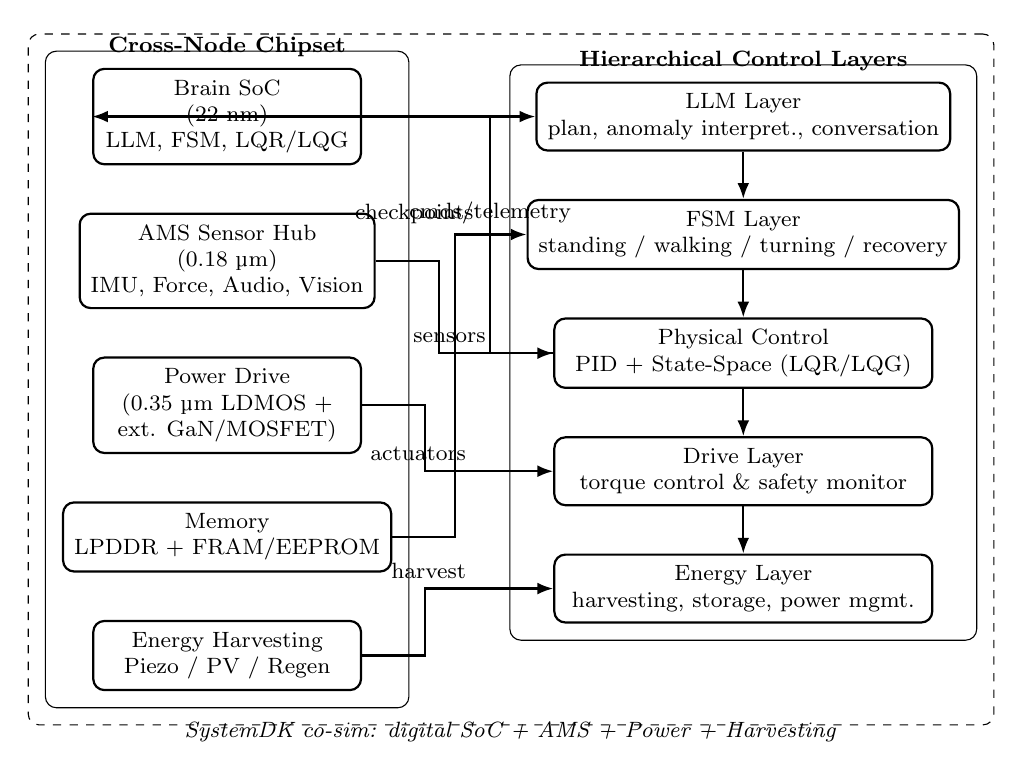
\begin{tikzpicture}[
  font=\footnotesize,
  >={Latex[length=2mm]},
  node distance=6mm and 6mm,
  box/.style={draw,rounded corners,thick,inner sep=4pt,align=center},
  grp/.style={draw,rounded corners,inner sep=6pt}
]
% 左:SoC/AMS/Power/Memory/Harvest
\node[box,minimum width=34mm,minimum height=8mm] (soc)
  {Brain SoC\\(22 nm)\\LLM, FSM, LQR/LQG};
\node[box,below=of soc,minimum width=34mm,minimum height=8mm] (ams)
  {AMS Sensor Hub\\(0.18 µm)\\IMU, Force, Audio, Vision};
\node[box,below=of ams,minimum width=34mm,minimum height=8mm] (pwr)
  {Power Drive\\(0.35 µm LDMOS +\\ ext. GaN/MOSFET)};
\node[box,below=of pwr,minimum width=34mm,minimum height=8mm] (mem)
  {Memory\\LPDDR + FRAM/EEPROM};
\node[box,below=of mem,minimum width=34mm,minimum height=8mm] (harv)
  {Energy Harvesting\\Piezo / PV / Regen};
\node[grp,fit=(soc)(ams)(pwr)(mem)(harv),
      label={[yshift=-2mm]above:\textbf{Cross-Node Chipset}}] (L) {};

% 右:制御レイヤ
\node[box,minimum width=48mm,minimum height=8mm, right=22mm of soc] (llm)
  {LLM Layer\\plan, anomaly interpret., conversation};
\node[box,below=of llm,minimum width=48mm,minimum height=8mm] (fsm)
  {FSM Layer\\standing / walking / turning / recovery};
\node[box,below=of fsm,minimum width=48mm,minimum height=8mm] (phys)
  {Physical Control\\PID + State-Space (LQR/LQG)};
\node[box,below=of phys,minimum width=48mm,minimum height=8mm] (drive)
  {Drive Layer\\torque control \& safety monitor};
\node[box,below=of drive,minimum width=48mm,minimum height=8mm] (energy)
  {Energy Layer\\harvesting, storage, power mgmt.};
\node[grp,fit=(llm)(fsm)(phys)(drive)(energy),
      label={[yshift=-2mm]above:\textbf{Hierarchical Control Layers}}] (R) {};

% 接続
\draw[thick,->] (soc.east) -- (llm.west);
\draw[thick,->] (llm.south) -- (fsm.north);
\draw[thick,->] (fsm.south) -- (phys.north);
\draw[thick,->] (phys.south) -- (drive.north);
\draw[thick,->] (drive.south) -- (energy.north);

\draw[thick,->] (ams.east) -- ++(8mm,0) |- (phys.west) node[pos=0.75,above left]{sensors};
\draw[thick,->] (pwr.east) -- ++(8mm,0) |- (drive.west) node[pos=0.7,above left]{actuators};
\draw[thick,->] (mem.east) -- ++(8mm,0) |- (fsm.west) node[pos=0.7,above left]{checkpoints};
\draw[thick,->] (harv.east) -- ++(8mm,0) |- (energy.west) node[pos=0.7,above left]{harvest};

\draw[thick,->] (phys.west) -- ++(-8mm,0) |- (soc.west)
  node[pos=0.25,above]{cmds/telemetry};

% SystemDK の囲み
\node[grp,dashed,fit=(L)(R),
  label={[yshift=2mm]below:\strut \textit{SystemDK co-sim: digital SoC + AMS + Power + Harvesting}}] {};
\end{tikzpicture}
%
  }{%
    \IfFileExists{figures/systemdk_flow.pdf}{%
      \includegraphics[width=\columnwidth]{figures/systemdk_flow.pdf}%
    }{%
      \fbox{\begin{minipage}[c][0.48\linewidth][c]{0.94\columnwidth}\centering
      \vspace{0.5em}\textit{Placeholder: \path{figures/systemdk_flow.{tikz|pdf}} not found}\\
      (Commit the figure to replace this box.)\vspace{0.5em}
      \end{minipage}}%
    }%
  }
  \caption{SystemDK-based integrated design flow spanning SoC (22 nm), AMS (0.18~µm),
    LDMOS power drive (0.35~µm), and energy harvesting subsystems.}
  \label{fig:systemdk_flow}
\end{figure}

\subsection{Key Performance Indicators}
The PoC architecture was evaluated against several key performance indicators (KPIs),
summarized in Table~\ref{tab:kpi_summary}. These metrics guided the design trade-offs
in posture recovery, gait stability, energy efficiency, and memory subsystem performance.

\begin{table}[t]
\caption{Summary of Key Performance Indicators (KPIs)}
\label{tab:kpi_summary}
\centering
\renewcommand{\arraystretch}{1.15}
\footnotesize
\begin{tabular}{@{}p{0.48\columnwidth} p{0.44\columnwidth}@{}}
\toprule
\textbf{Metric} & \textbf{Result} \\
\midrule
Posture recovery time & $\leq 200$ ms (vs.\ $>500$ ms with PID only) \\
Gait stability (CoM RMS) & $\approx 30\%$ improvement over PID only \\
Energy efficiency & $+15\%$ with hybrid control + harvesting \\
Self-harvest contribution & Up to $20\%$ of power budget \\
Checkpoint resume time & $\leq 10$ ms (FRAM/EEPROM) \\
Memory endurance & $10^{12}$ write cycles \\
\bottomrule
\end{tabular}
\end{table}

\section{Results and Discussion}
System-level simulation was performed with representative AI inference workloads.

\subsection{Standby Power}
Migrating cold data and checkpoints to the FeRAM-backed tier yields more than 30\% reduction in standby power.
This reduction arises from suppressing periodic DRAM refresh for inactive regions.

\subsection{Resume Latency}
FeRAM allows direct restore of checkpoints without full DRAM wake-up.
Resume latency is reduced to the $\mu$s range, enabling near-instant resume after power gating and improving energy efficiency for mobile edge AI.

\subsection{Endurance}
FeRAM endurance of $10^{12}$~writes/year fits within FeRAM capability for checkpoint traffic.

% ===== Fig.2: Access time vs. Retention =====
\begin{figure}[!t]
\centering
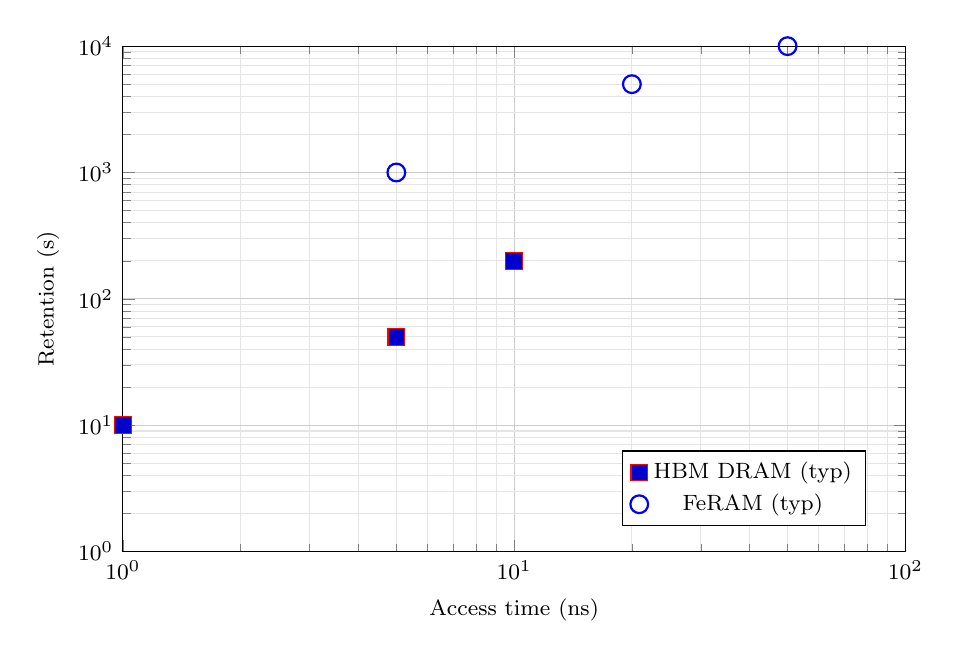
\begin{tikzpicture}
\begin{axis}[
    width=0.95\linewidth,   % 横幅をページ幅の95%に拡大
    height=8cm,             % 高さも拡大
    xlabel={Access time (ns)},
    ylabel={Retention (s)},
    xmode=log, ymode=log,
    xmin=1e0, xmax=1e2,
    ymin=1e0, ymax=1e4,
    grid=both,
    major grid style={gray!40},
    minor grid style={gray!20},
    legend style={
        at={(0.95,0.05)},     % グラフの右下
        anchor=south east,
        font=\footnotesize,
        fill=white,
        draw=black
    },
    tick label style={font=\footnotesize},
    label style={font=\footnotesize}
]

% HBM: 赤四角
\addplot+[only marks, mark=square*, mark size=3pt, red]
coordinates {(1, 10) (5, 50) (10, 200)};

% FeRAM: 青丸
\addplot+[only marks, mark=o, mark size=3.2pt, blue, thick]
coordinates {(5, 1e3) (20, 5e3) (50, 1e4)};

\legend{HBM DRAM (typ), FeRAM (typ)}
\end{axis}
\end{tikzpicture}
\caption{Access time vs. retention. Red squares: HBM; blue circles: FeRAM. Wider and taller view for clarity ($10^0$--$10^2$ ns, $10^0$--$10^4$ s).}
\label{fig:retention}
\end{figure}

\section{Discussion}
Table~\ref{tab:humanoid_comparison} compares the proposed Samizo-AITL PoC
with two representative humanoid platforms: Boston Dynamics \textit{Atlas} 
and Tesla \textit{Optimus}.
Atlas excels at dynamic acrobatics, while Optimus emphasizes scalable
industrial deployment. In contrast, the proposed PoC targets autonomy,
fault tolerance, and sustainable operation.

A first distinctive feature is the integration of LLMs into the hierarchical
control loop. Instead of replacing classical controllers, the LLM layer
generates goals, interprets anomalies, and provides conversational interfaces.
This complements the FSM for supervisory logic and PID/state-space methods
for stabilization, creating a hybrid architecture that combines the safety
of model-based control with the adaptability of data-driven intelligence.

A second differentiator is energy autonomy. The PoC integrates
piezoelectric, photovoltaic, and regenerative harvesting,
allowing up to 20\% of the power budget to be sustained
without external charging. This contrasts with Atlas and Optimus,
which rely exclusively on batteries. Together with FRAM/EEPROM-based
checkpoint-and-resume, the system ensures resilient operation
in remote or resource-limited environments.

A third contribution is educational reproducibility.
All specifications, models, and proof-of-concept results are openly published
in bilingual (Japanese–English) format on GitHub Pages.
This open-science approach enables replication, lowers barriers for students,
and positions the PoC as both a research prototype and an instructional
benchmark in control engineering education.

Overall, the proposed system demonstrates that hybrid architectures
can extend humanoid robotics beyond performance and manufacturability,
toward autonomy, resilience, and sustainable deployment.

\section{Conclusion}
This paper has proposed a Bio-Inkjet (Bio-IJ) architecture based on
bulk KNN actuators as a lead-free alternative to conventional PZT-based
printheads.
By combining multilayer KNN stacks, COF driver ICs, and silicon cavity
integration, the system achieves picoliter-scale droplet generation
under moderate voltages while ensuring material biocompatibility.

Unlike industrial printing, where full PZT compatibility in terms of
maximum $d_{33}$, billion-cycle endurance, and cost efficiency is
required, biomedical printing places emphasis on safety, controlled
droplet volume, and operational reliability over shorter lifetimes.
The proposed approach aligns well with these requirements, providing
sufficient performance for applications such as cell patterning,
protein microarrays, and hydrogel 3D fabrication.

These findings highlight bulk KNN as a practical foundation for
standardizing lead-free Bio-IJ systems in research, clinical, and
educational domains.
Future work will involve experimental validation of droplet formation,
long-term reliability testing under bio-relevant conditions, and system
integration with existing bioprinting workflows.

\textbf{Most importantly, this work emphasizes that in biomedical inkjet
printing, safety and biocompatibility must take precedence over extreme
performance metrics, positioning KNN-based Bio-IJ as a safe and viable
path toward Pb-free bioprinting.}


% ===== Acknowledgment =====
\section*{Acknowledgment}
The author would like to thank the open-source community and educational collaborators
who contributed to the EduController, Edusemi, and AITL projects,
which formed the foundation of this work.

% ===== References =====
\bibliographystyle{IEEEtran}
\nocite{*}  % ★ refs.bib の全エントリを出力(エラー回避)
\bibliography{refs}

% ===== Author Biography =====
\vspace{-0.5\baselineskip}
\begingroup\small
\begin{IEEEbiographynophoto}{Shinichi Samizo}
received the M.S. degree in Electrical and Electronic Engineering from Shinshu University, Japan.
He worked at Seiko Epson Corporation as an engineer in semiconductor memory and mixed-signal device development, and also contributed to inkjet MEMS actuators and PrecisionCore printhead technology.
He is currently an independent semiconductor researcher focusing on process/device education, memory architecture, and AI system integration.

\textbf{Contact:} \href{mailto:shin3t72@gmail.com}{shin3t72@gmail.com},
\href{https://github.com/Samizo-AITL}{Samizo-AITL}
\end{IEEEbiographynophoto}
\endgroup

\end{document}
